\documentclass{article}
\usepackage{fancyhdr}
\usepackage{lastpage}
\usepackage{amsmath}
\usepackage{amssymb}
\usepackage{amsthm}
\usepackage{tabstackengine}
\usepackage[margin=1in]{geometry}
\usepackage{graphicx}
\graphicspath{ {./} }
\TABstackMath
\TABbinary

\pagestyle{fancy}
\setlength\headheight{28pt}
\addtolength{\headheight}{\baselineskip}
\fancyhf{}
\renewcommand{\headrulewidth}{0pt}
\lhead{Math 251 - Shuichi Masuda\\Juno Suárez\\\today}
\rfoot{Page \thepage \hspace{1pt} of \pageref{LastPage}}

\renewcommand\thesubsection{\arabic{subsection}.}
\renewcommand\thesubsubsection{\alph{subsubsection})}

\begin{document}

\section*{Graded Problems \# 3}

\subsection{}
For this problem, I'm assuming no air resistence and the constant acceleration of gravity of $g = 9.8\text{m/s}^2$. Since the problem specifies that the rock is thrown straight up, I'll model its height as position along a single axis, $s$, as a function dependent on time $t$, using the position function. The height of the ground below the cliff will be set to 0, so the height of the cliff above the ground will be a positive value between 0 and the maximum height at time $t=2$ given by $s(2)$.
\\

We're trying to find the following unknowns:
\begin{itemize}
\item Initial velocity of the rock: $v_{0}$
\item Height of the cliff above the ground: $s(0)$ or $s_{0}$
\item Velocity of the rock at time $t$: $v(t)$
\item Velocity of the rock when it hits the ground: $v(7)$
\end{itemize}

$$
s(t) = s_{0} + v_{0}t - \frac{1}{2}gt^2
$$

We can sketch the graph of this function:

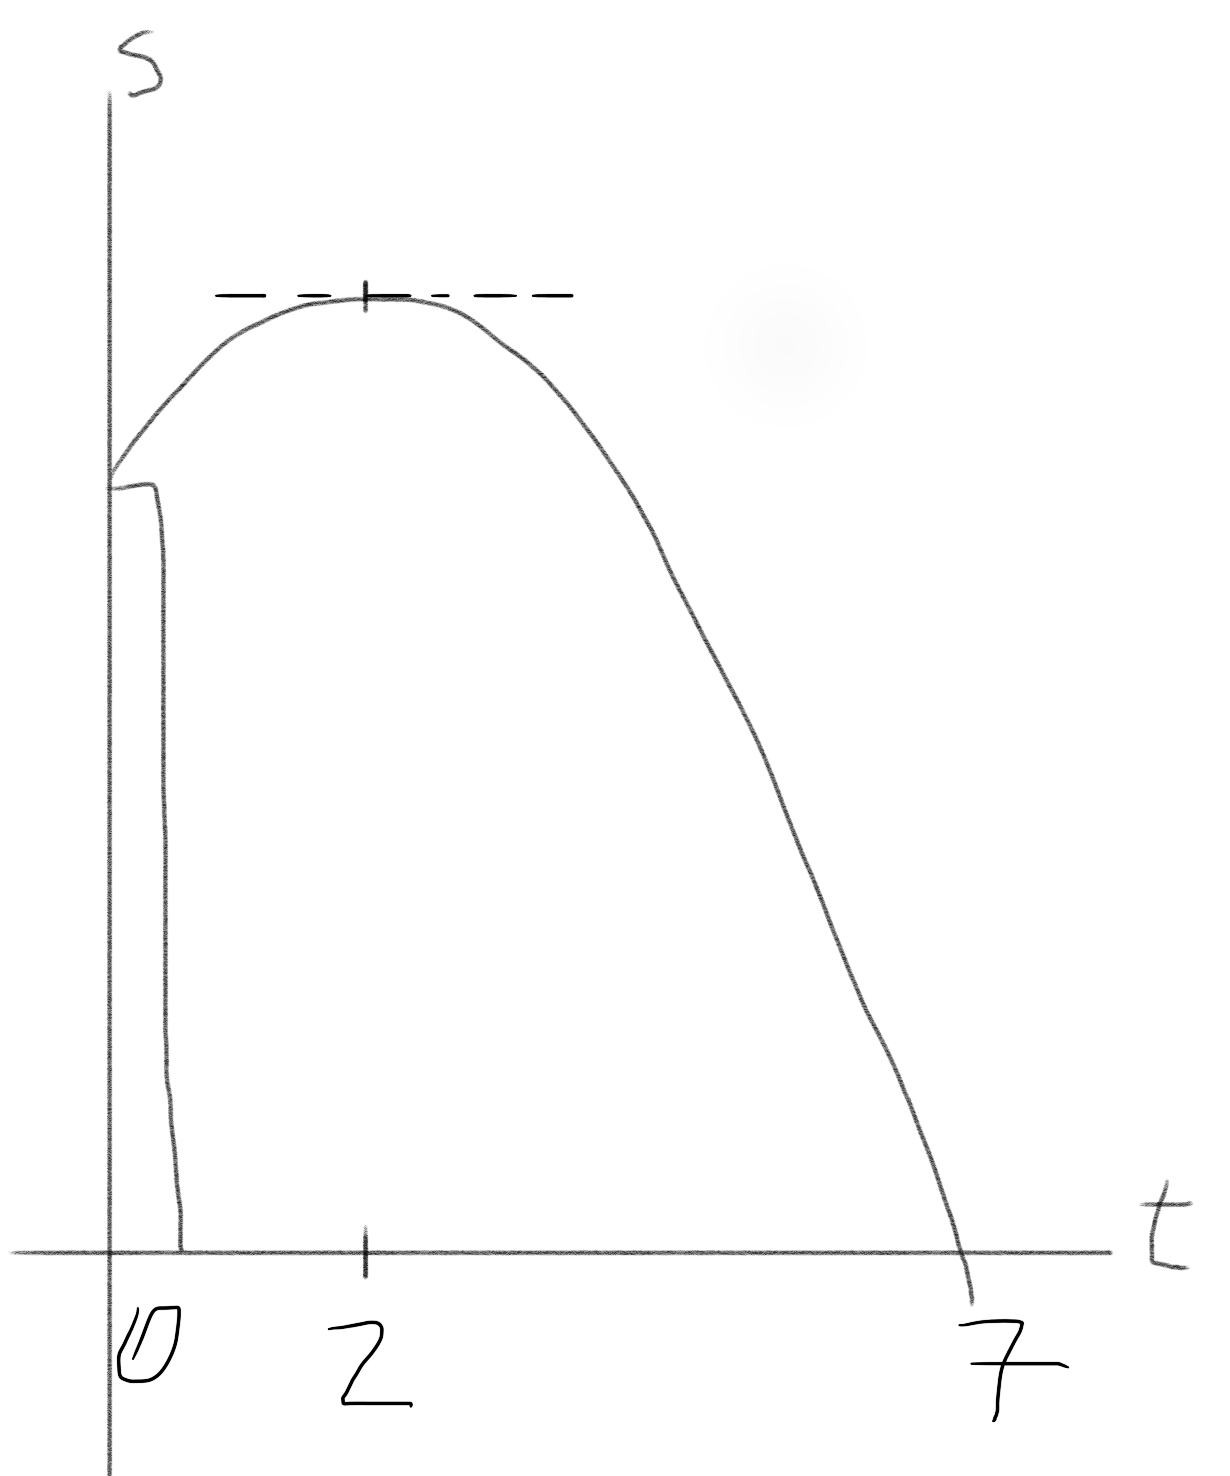
\includegraphics[height=3in]{gp3-sketch}

The velocity function can be derived by taking the derivative of the position function. We can find the general form before solving for the constants $s_{0}$ or $v_{0}$:
\\

\tabbedLongunderstack[l]{
  v(t) = \frac{d}{dt}s(t) \\
  \\
  \phantom{v(t)} = \boxed{v_{0} - gt}
}
\Longunderstack[l]{
  Power rule \\
}
\\

We know from Galileo (if not from my drawing skills) that the trajectory of this function is a parabola. The maximum height, at $t=2$, is the vertex of this parabola. At this point, the slope of the tangent is 0. Therefore, $v(2)=0$. With this, we can solve for $v_{0}$:
\\

\tabbedLongunderstack[l]{
  0 = v_{0} - g2\\
  \boxed{v_{0} = 2g}
}
\Longunderstack[l]{
  \:\: Add g2 to both sides and rewrite \\
}
\\


With that, our velocity fuction is
$$
\boxed{v(t) = 2g - gt}
$$

And we can solve for the velocity of the rock when it hits the ground,
$$
v(7) = 2g - g\cdot(7) = \boxed{-5g}
$$

Knowing the initial velocity, we can solve for the height of the cliff. In our frame of reference, we've set ground level to 0, so $s(7) = 0$. We solve for $s_{0}$:
\\

\tabbedLongunderstack[l]{
  0 = s_{0} + 2g \cdot 7 - \frac{1}{2}g \cdot 7^2\\
  -s_0 = \frac{28}{2}g - \frac{49}{2}g\\
  -s_0 = -\frac{21}{2}g\\
  \\
  \boxed{s_0 = \frac{21}{2}g}\\
}
\Longunderstack[l]{
}
\\

Finally, we can report our results:


\begin{itemize}
  \item Initial velocity of the rock: $\boxed{v_{0} = 2g} \text{ or } \approx 19.6\text{m/s}$.
  \item Height of the cliff above the ground: $\boxed{s(0) = \frac{21}{2}g} \text{ or } \approx 102.9\text{m}$.
  \item Velocity of the rock at time $t$: $\boxed{v(t) = 2g - gt}$
  \item Velocity of the rock when it hits the ground: $\boxed{v(7) = -5g} \text { or } \approx -49\text{m/2}$.
\end{itemize}

\subsection{}
See attached.


\end{document}
